% Figure from MATH 556 notes, section 33. Compile with the notes preamble.
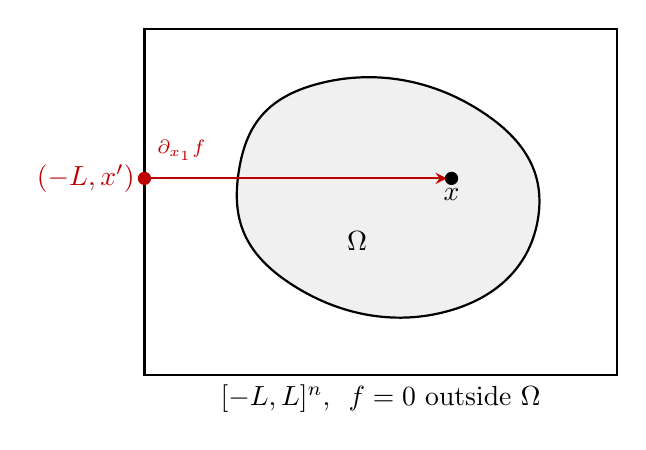
\begin{tikzpicture}[scale=2.0, >=stealth]
    \draw[thick] (-1.5,-1.1) rectangle (1.5,1.1);
    \draw[thick, fill=gray!12] plot[smooth cycle, tension=0.8] coordinates {(-0.9,0.2) (-0.4,0.75) (0.6,0.6) (1.0,-0.1) (0.4,-0.7) (-0.6,-0.5)};
    \node at (-0.15,-0.25) {$\Omega$};
    \fill (0.45,0.15) circle (1.2pt) node[below] {$x$};
    \draw[->, red!75!black, thick] (-1.5,0.15) -- (0.42,0.15);
    \fill[red!75!black] (-1.5,0.15) circle (1.2pt);
    \node[red!75!black, left] at (-1.5,0.15) {$(-L, x')$};
    \node[red!75!black, anchor=south west, font=\scriptsize] at (-1.48,0.2) {$\partial_{x_1} f$};
    \node[below] at (0,-1.1) {$[-L, L]^n$, \ $f = 0$ outside $\Omega$};
\end{tikzpicture}
